%%%% A summary of basic Markov decision theory.

% Plain and simple
\documentclass{article}

% Format and figure stuff
\usepackage{geometry}
\usepackage{graphicx}
\usepackage{float}
\usepackage[usenames, dvipsnames]{color}

% Text stuff
\usepackage{tikzsymbols}

% Math stuff
\usepackage{mathtools}
\usepackage{mathrsfs}
\usepackage{amsmath}
\usepackage{amssymb}
\usepackage{cancel}
\usepackage{xfrac}
\usepackage{bm}

% Code stuff
\usepackage{listings}
\usepackage{hyperref}

% Page layout
\geometry{top=1in,bottom=1in}
\hyphenpenalty = 10000
\setlength\parindent{0pt}
\setlength{\jot}{10pt}

% Hyperlink format
\hypersetup{colorlinks=true,
            linkcolor=blue,
            filecolor=magenta,
            urlcolor=blue}

% Tab command
\newcommand\tab[1][1cm]{\hspace*{#1}}

% Line command
\newcommand\myline{\noindent\makebox[\linewidth]{\rule{\paperwidth - 2in}{0.4pt}}}

% Code font
\def\code#1{\texttt{#1}}

% Quick colors
\definecolor{stateblue}{rgb}{0, 0, 0.75}
\definecolor{darkgreen}{rgb}{0, 0.5, 0}
\definecolor{orange}{RGB}{180, 60, 0}
\definecolor{purple}{RGB}{200, 0, 200}
\def\green#1{\textcolor{darkgreen}{#1}}
\def\red#1{\textcolor{red}{#1}}
\def\blue#1{\textcolor{stateblue}{#1}}
\def\orange#1{\textcolor{orange}{#1}}
\def\purple#1{\textcolor{purple}{#1}}
\def\black#1{\textcolor{black}{#1}}

% Coordinate system notation
\def\cs#1#2%
  {\mathop{}%
   \mathopen{\vphantom{#2}}^{#1}%
   \kern-\scriptspace%
   #2}

% Custom math symbols - linear algebra
\DeclareMathOperator*{\tr}{\intercal}
\DeclareMathOperator*{\zero}{\underline{0}}
\DeclareMathOperator*{\eye}{\underline{1}}
\newcommand\inv[1]{#1\raisebox{1.15ex}{$\scriptscriptstyle-\!1$}}
\newcommand\pinv[1]{#1\raisebox{1.15ex}{$\scriptscriptstyle\dist\!1$}}

% Custom math symbols - probability
\DeclareMathOperator*{\E}{E}
\DeclareMathOperator*{\cov}{cov}
\DeclareMathOperator*{\dist}{\sim}
\DeclareMathOperator*{\argmin}{arg\,min}
\DeclareMathOperator*{\argmax}{arg\,max}


\begin{document}

%%%%%%%%%%%%%%%%%%%%%%%%%%%%%%%%%%%%%%%%%%%%%%%%% TITLE

\title{\textbf{Markov Decision Processes}\\ \large{A Reasonably Precise Summary}\vspace{-6ex}}
\author{\vspace{-5ex}}
\date{\small{Jason Nezvadovitz -- February 2020}}
\maketitle

%%%%%%%%%%%%%%%%%%%%%%%%%%%%%%%%%%%%%%%%%%%%%%%%% BODY

The purpose of this document is to provide a succinct, mathematically precise summary of basic Markov decision theory for review. The focus is on axiomatic clarity rather than intuition. The reader should already have a good understanding of probability theory and basic machine learning.

\vspace{0.2in}
\hrule
\vspace{0.2in}

Declare ``time'': a countable set $\mathbb{T} \coloneqq \{0, 1, 2, \cdots, n\}$ for some potentially infinite ``horizon'' $n$.\\
Denote a generic element as $t \in \mathbb{T}$.\\

In the most general setting, time can be continuous (uncountable), but we will restrict ourselves to discrete time here to avoid the complications of stochastic calculus.\\

Declare the ``state space'': a set $\mathbb{S}$ of any cardinality. Could be $\mathbb{R}^2$, $\{\text{\Smiley},\text{\Cooley},\text{\Winkey}\}$, whatever.\\
Denote a generic element as $s \in \mathbb{S}$.\\

Declare the ``action space'': a set $\mathbb{A}$ of any cardinality. No restrictions.\\
Denote a generic element as $a \in \mathbb{A}$.\\

We will now build a standard \href{https://en.wikipedia.org/wiki/Probability_space}{probability space}, $\boldsymbol{(}\Omega, \mathcal{F}, P\boldsymbol{)}$.\\

Let the sample space be \ $\Omega \coloneqq \mathbb{S}^{n+1} \times \mathbb{A}^n \times \mathbb{R}^n$.\\
An individual sample $\omega \in \Omega$ is called a ``trajectory.''\\

Each trajectory consists of an ``initial condition'' $s_0$, and $n$ triplets of the form $(a_t, s_{t+1}, r_{t+1})$ called ``transitions,'' where the $r \in \mathbb{R}$ are called ``rewards.'' I.e.,
\begin{equation*}
\omega \coloneqq \{s_0, (a_0, s_1, r_1), (a_1, s_2, r_2), \cdots, (a_{n-1}, s_{n}, r_n)\}
\end{equation*}

Let the event set $\mathcal{F}$ be the product sigma-algebra of $\Omega$, using the Borel sigma-algebra for uncountable sets and the power-set sigma-algebra for countable sets.\\

Define the probability measure $P : \mathcal{F} \to [0,1]$ in terms of the distribution $p : \Omega \to \mathbb{R}_+$ by sums,
\begin{equation*}
P(B) \coloneqq \int_B p(\omega)\, d\omega\ \ \forall B \in \mathcal{F},\ \ \text{where}\ \ p(\omega)\geq0\ \ \text{and}\ \ \int_\Omega p(\omega)\,d\omega = 1
\end{equation*}

We declare $p$ to have ``Markovian'' structure, i.e. the following factorization:
\begin{align*}
p(\omega) &= p(s_0, a_0, s_1, r_1, a_1, s_2, r_2, \cdots, a_{n-1}, s_{n}, r_n)\\
&\stackrel{\text{markov}}{\coloneqq}\ p(s_0) \prod_{t=0}^{n-1} \red{p(a_t|s_t)}\blue{p(s_{t+1}|s_t,a_t)}\green{p(r_{t+1}|s_t,a_t,s_{t+1})}
\end{align*}

where we are using the usual overloaded notation for marginal and conditional distributions,\\
\begin{equation*}
p(x) \coloneqq \int p(x,y)\,dy\ \ \ \text{and}\ \ \ p(x|y) \coloneqq \frac{p(x,y)}{p(y)}
\end{equation*}

Practically speaking, the Markov property allows us to completely define high-dimensional trajectory probability densities $p(\omega)$ by specifying just the following lower-dimensional distributions:
\begin{itemize}
  \item The ``initial condition'' $p(s_0)$
  \item The ``\red{policies}'' $\red{p(a_t|s_t)}\ \forall t$
  \item The ``\blue{dynamics}'' $\blue{p(s_{t+1}|s_t,a_t)}\ \forall t$
  \item The ``\green{rewards}'' $\green{p(r_{t+1}|s_t,a_t,s_{t+1})}\ \forall t$
\end{itemize}

If, for example, the expression of $p(a_t|s_t)$ does not depend explicitly on the time index $t$, then we say there is just one ``policy'' (nonplural) and that it is ``time invariant.'' It is often the case that all of the above are time invariant, and so we really only have one unique policy, one unique dynamic, and one unique reward distribution that are just replicated $n$-times in the factorization of $p(\omega)$.\\

Also, whenever a distribution's form is that of a Dirac/Kronecker-delta, we call it ``deterministic'' instead of ``stochastic.'' It is common for both the policies and rewards to be deterministic. In fact, the reward distribution is often deterministic, time invariant, and even independent of $s_{t+1}$, meaning that it can be fully specified by a single function $\bar{r}:\mathbb{S}\times\mathbb{A} \to \mathbb{R}$ through,
\begin{equation*}
p(r_{t+1}|s_t,a_t,s_{t+1}) = \delta\big{(}r_{t+1} - \bar{r}(s_t, a_t)\big{)} \tag{\small{deterministic reward}}
\end{equation*}

Anyway, the Markov property implies many strong conditional independence statements. E.g.,
\begin{equation*}
p(s_{t+1}|s_t,a_t,s_{t-1},a_{t-1},r_{t-1},s_{t-2},a_{t-2},r_{t-2},\cdots) = p(s_{t+1}|s_t,a_t)
\end{equation*}

These relationships can be depicted succinctly via a \href{https://en.wikipedia.org/wiki/Bayesian_network}{Bayesian graph} over the convenience random variables \ ${s_t}(\omega) \coloneqq s_t$, \ ${a_t}(\omega) \coloneqq a_t$, \ and \ ${r_t}(\omega) \coloneqq r_t$.
\begin{center}
  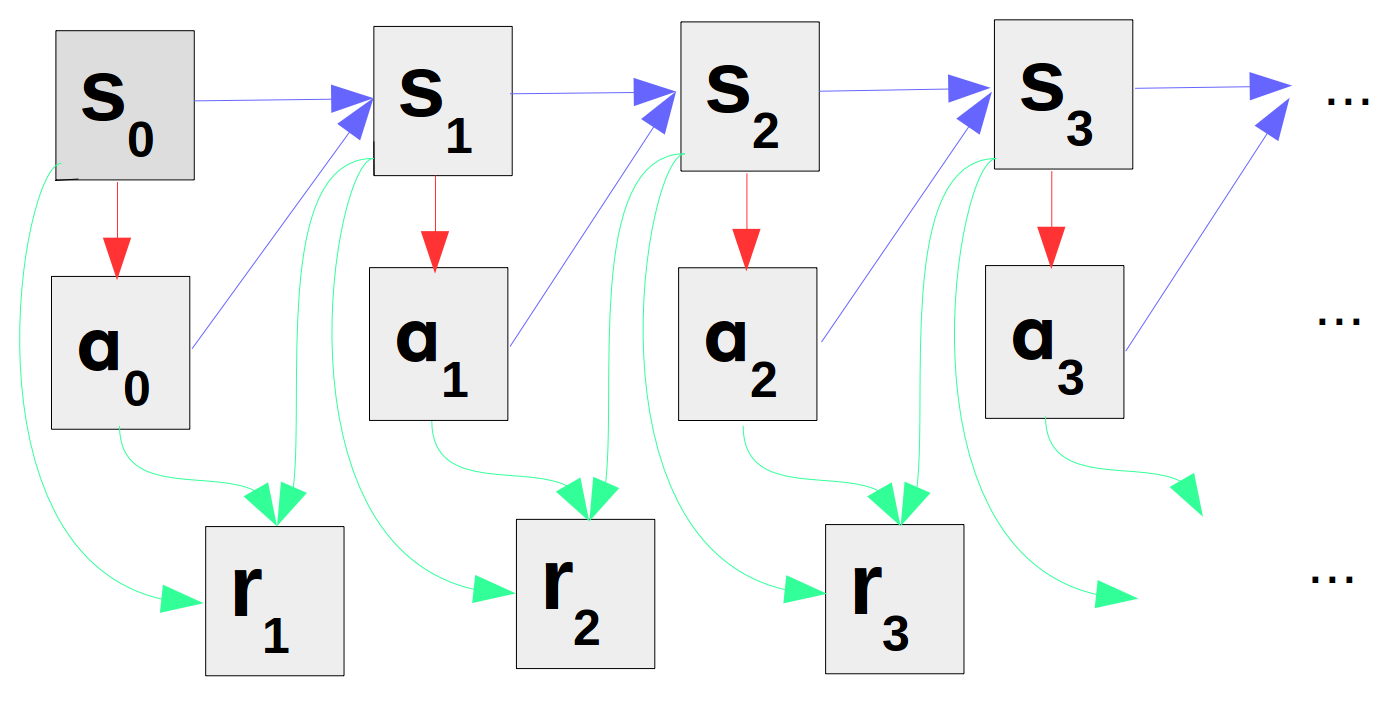
\includegraphics[width=\linewidth-1.5in]{include/bayesian_graph.png}
\end{center}

This temporally ``chained'' structure models the idea that ``given the present, the future is independent of the past'' and constitutes the entirety of a ``Markov decision process'' (MDP). Specifically, if we define the random variable $\omega_t$ to be the elements of a trajectory for times $\tau \geq t$ (``the future''),
\begin{equation*}
\omega_t \coloneqq \{s_t, (a_t, s_{t+1}, r_{t+1}), (a_{t+1}, s_{t+2}, r_{t+2}), \cdots, (a_{n-1}, s_{n}, r_n)\} \ \in \ \Omega_t \coloneqq \mathbb{S}^{n-t+1} \times \mathbb{A}^{n-t} \times \mathbb{R}^{n-t}
\end{equation*}

we see from the Bayesian graph that $\omega_t$ is disconnected from ``the past'' by conditioning on $s_t$,
\begin{equation*}
p(\omega_t|s_t) = \cancel{\frac{p(s_t)}{p(s_t)}}\prod_{\tau=t}^{n-1} p(a_\tau|s_\tau)p(s_{\tau+1}|s_\tau,a_\tau)p(r_{\tau+1}|s_\tau,a_\tau,s_{\tau+1})
\end{equation*}

We now define the ``total (discounted) reward from $t$'' to be a random variable that assesses the goodness of a sample of our MDP starting from time $t$ by summing up the remaining rewards,
\begin{align*}
G_t(\omega_t) &\coloneqq r_{t+1} + \gamma r_{t+2} + \gamma^2 r_{t+3} + \cdots + \gamma^{n-t-1} r_n\\
&= \sum_{\tau=t}^{n-1} \gamma^{\tau-t} r_{\tau+1}
\end{align*}

where $\gamma \in [0,1]$ is called the ``discount factor,'' used both to enforce the convergence of this sum (if $n \to \infty$) and to express that future rewards are less valuable than sooner rewards.\\

Total reward provokes an optimization problem: we want to choose the best possible policy distribution $p(a_t|s_t)$. To clarify, the ``decision'' in ``Markov decision process'' is really deciding the distribution from which actions will be sampled (the policy). If the policy depends only on time (ignoring the actual value of $s$) we call it ``open-loop'' or a ``plan,'' while if it depends on $s$ in any way we call it ``closed-loop.'' If the policy is deterministic and time invariant, then it can be fully specified by a single function $\mathbb{S} \mapsto \mathbb{A}$ that is interpreted classically as a decision-making rule.\\

We will denote our choice as $\pi(a_t|s_t)$, and to emphasize that we have plugged-in our choice, we will use $\pi$ as a subscript on probability densities and statistics. For example,
\begin{equation*}
p_{\orange{\pi}}(\omega) \coloneqq p(\omega)\Big{|}_{p(a_t|s_t) = \orange{\pi(a_t|s_t)}} = p(s_0) \prod_{t=0}^{n-1} \orange{\pi(a_t|s_t)}p(s_{t+1}|s_t,a_t)p(r_{t+1}|s_t,a_t,s_{t+1})
\end{equation*}

But what exactly does ``best'' mean with respect to a random variable like $G_t$? We choose to optimize a statistic of $G_t$. Namely, a conditional expectation called the ``value function,''
\begin{align*}
V_\pi(s_t) &\coloneqq E_\pi(G_t | s_t)\\
&= \int_{\Omega_t} G_t(\omega_t) p_\pi(\omega_t|s_t)\,d\omega_t\\
&= \int_{\Omega_t} \sum_{\tau=t}^{n-1} \Big{(}\gamma^{\tau-t} r_{\tau+1}\Big{)} \prod_{\tau=t}^{n-1} \Big{(}\pi(a_\tau|s_\tau)p(s_{\tau+1}|s_\tau,a_\tau)p(r_{\tau+1}|s_\tau,a_\tau,s_{\tau+1})\Big{)} \,d\omega_t
\end{align*}

So $V_\pi(s_t)$ is the expected total reward acquired for starting from state $s$ at time $t$ and acting according to policy $\pi$. Our objective then is to find the optimal policy $\pi^*$ that satisfies,
\begin{equation*}
V_{\pi^*}(s_t) \geq V_{\pi}(s_t)\ \forall s_t
\end{equation*}

There is a necessary and sufficient condition for $\pi^*$ known as the ``dynamic programming principle'':
\begin{quote}
``An optimal policy has the property that, whatever the initial state and initial action are, the remaining actions must constitute an optimal policy with regard to the state resulting from the first action.'' (Bellman, 1957, Chapter III.3)
\end{quote}

This follows directly from the Markov property: given that the process is now in state $s_{t+1}$, the future of the process is independent of how it got there (i.e. the transition from $s_t$ using $a_t$). Therefore, if we can predict the optimal outcome from any $s_{t+1}$, then we can determine $\pi^*(a_t|s_t)$ by optimizing just the expected immediate reward plus our prediction for the optimal outcome from the states we might transition to (discounted by $\gamma$ since it's future reward). Said mathematically,
\begin{gather*}
\pi^*(a_t|s_t) = \delta\big{(}a_t\ ;\ \bar{\pi}^*(s_t)\big{)}\\
\bar{\pi}^*(s_t) = \argmax_{a_t} E\big{(}r_{t+1} + \gamma V_{\pi^*}(s_{t+1}) | s_t, a_t\big{)}
\end{gather*}

However, this only gives us $\pi^*$ in terms of $V_{\pi^*}$ which we still don't know. To resolve this, consider the following recursion satisfied by the total reward,
\begin{align*}
G_t &= r_{t+1} + \gamma \big{(}r_{t+2} + \gamma r_{t+3} + \cdots + \gamma^{n-t-2} r_n\big{)}\\
&= r_{t+1} + \gamma G_{t+1}
\end{align*}

and the following properties of expectation for any random variables $x$, $y$, and $z$,
\begin{align*}
E(\alpha x + \beta y) &= \alpha E(x) + \beta E(y)\\
E(x | z) &= E\big{(}E(x | y, z) | z\big{)}
\end{align*}

It follows that any value function also satisfies a recursion,
\begin{align*}
V_\pi(s_t) &= E_\pi(r_{t+1} + \gamma G_{t+1} | s_t)\\
&= E_\pi(r_{t+1}|s_t) + \gamma E_\pi(G_{t+1} | s_t)\\
&= E_\pi(r_{t+1}|s_t) + \gamma E_\pi\big{(}E_\pi(G_{t+1}|s_{t+1},s_t) | s_t\big{)}\\
&= E_\pi(r_{t+1}|s_t) + \gamma E_\pi\big{(}V_{\pi}(s_{t+1}) | s_t\big{)}\\
&= E_\pi\big{(}r_{t+1} + \gamma V_{\pi}(s_{t+1}) | s_t\big{)}
\end{align*}

And, since there is no more reward to be collected after time $n$, we have a boundary condition,
\begin{equation*}
V_{\pi}(s_n) = 0
\end{equation*}

Plugging-in the dynamic programming principle's $\pi^*$, we arrive at the ``Bellman equation'':
\begin{equation*}
V^*(s_t) = \max_{a_t} E\big{(}r_{t+1} + \gamma V^*(s_{t+1}) | s_t, a_t\big{)}
\end{equation*}

with the shorthand $V^* \coloneqq V_{\pi^*}$. If we can solve the Bellman equation for $V^*$, then $\pi^*$ can be reconstructed as the deterministic policy that always selects the $\argmax$ of the right-hand-side. Thus, a solution $V^*$ to the Bellman equation constitutes a solution to our MDP.\\

It is worth noting that the general value function recursion is useful for more than just deriving the Bellman equation. It lets us compute the value function associated with any policy, which can be useful when comparing candidate policies if the Bellman equation is too difficult to solve directly. The general value function recursion doesn't involve the difficult maximization present in the Bellman equation and is thus linear in the unknown $V_\pi$.\\

The expectations in these equations pack away a lot of computation, though they're not as intense as the expectation in the direct expression of $E_\pi(G_t|s_t)$, because the arguments of these expectations depend only on a single transition, not a whole trajectory, so we only need,
\begin{equation*}
p_\pi(a_t, s_{t+1}, r_{t+1}|s_t) = \orange{\pi(a_t|s_t)} \blue{p(s_{t+1}|s_t,a_t)} \green{p(r_{t+1}|s_t,a_t,s_{t+1})}
\end{equation*}

to express the general value function recursion as,
\begin{align*}
V_\pi(s_t) &= E_\pi\big{(}r_{t+1} + \gamma V_{\pi}(s_{t+1}) | s_t\big{)}\\
&= \orange{\int_{\mathbb{A}} \pi(a_t|s_t) \blue{\int_{\mathbb{S}} p(s_{t+1}|s_t,a_t) \Big{(}\green{\int_{\mathbb{R}}p(r_{t+1}|s_t,a_t,s_{t+1}) r_{t+1} \,dr_{t+1}} + \gamma V_{\pi}(s_{t+1}) \Big{)}\,ds_{t+1}}\,da_t}
\end{align*}

and similarly express the Bellman equation as,
\begin{align*}
V^*(s_t) &= \max_{a_t} E\big{(}r_{t+1} + \gamma V^*(s_{t+1}) | s_t, a_t\big{)}\\
&= \orange{\max_{a_t} \blue{\int_{\mathbb{S}} p(s_{t+1}|s_t,a_t) \Big{(}\green{\int_{\mathbb{R}} p(r_{t+1}|s_t,a_t,s_{t+1})r_{t+1} \,dr_{t+1}} + \gamma V^*(s_{t+1}) \Big{)}\,ds_{t+1}}}
\end{align*}

This is the most general case for a (vanilla) MDP, but there are many very common situations that simplify things. For example, if the reward is deterministic and independent of $s_{t+1}$, it can be pulled out of the $\mathbb{R}$ and $\mathbb{S}$ integrations to write the Bellman equation as,
\begin{equation*}
V^*(s_t) = \max_{a_t} \big{(} \bar{r}(s_t, a_t) + \gamma \mathcal{T}_{a_t} V^*(s_t) \big{)} \tag{\small{deterministic reward}}
\end{equation*}

with the linear ``transition operator'' defined as,
\begin{align*}
\mathcal{T}_{a_t} f(s_t) &\coloneqq E\big{(}f(s_{t+1})|s_t,a_t\big{)}\ \ \ \ \forall f : \mathbb{S} \times \mathbb{T} \to \mathbb{R}\\
&= \int_{\mathbb{S}}p(s_{t+1}|s_t,a_t)f(s_{t+1})\,ds_{t+1}
\end{align*}

Furthermore, if the MDP is fully time invariant (thus infinite horizon) and has finite state and action spaces, the above reduces to the form that is often presented first in introductory texts,
\begin{equation*}
V^*(s) = \max_{a} \Big{(} \bar{r}(s, a) + \gamma \sum_{s' \in \mathbb{S}} p(s'|s,a) V^*(s') \Big{)} \tag{\small{deterministic reward, time invariant, finite}}
\end{equation*}

which can be readily implemented as matrix operations on the value function as a single finite vector. It is also worth noting that if the dynamics are deterministic, the sum on the right reduces to a simple evaluation of $V^*$ at the only state $s'$ deterministically transitioned to from $s$ using $a$,
\begin{equation*}
V^*(s) = \max_{a} \Big{(} \bar{r}(s, a) + \gamma V^*\big{(}\bar{s}'(s, a)\big{)} \Big{)} \tag{\small{fully deterministic, time invariant, finite}}
\end{equation*}

In general, the Bellman equation is just a fixed-point equation for the nonlinear ``Bellman operator,''
\begin{gather*}
V^*(s_t) = \mathcal{B}V^*(s_t)\\
\mathcal{B} f(s_t) \coloneqq \max_{a_t} E\big{(}r_{t+1} + \gamma f(s_{t+1}) | s_t, a_t\big{)}\ \ \ \ \forall f : \mathbb{S} \times \mathbb{T} \to \mathbb{R}
\end{gather*}

It can be shown that \href{https://people.eecs.berkeley.edu/~ananth/223Spr07/ee223_spr07_lec19.pdf}{the Bellman operator is a contraction mapping}. Thus a variety of fixed-point-iteration-type algorithms can be used to numerically solve the Bellman equation with guaranteed convergence. In ``value iteration,'' the value of $\mathcal{B}\hat{V}^*(s_t)$ is simply used as the next iterate for $\hat{V}^*(s_t)$.
\begin{align*}
&\text{Guess}\ \ \hat{V}^*_0\\
&\forall\ i \in \mathbb{N}\ :\\
&\text{\tab} \forall\ s_t \in {\mathbb{S} \times \mathbb{T}}\ :\\
&\text{\tab \tab Recurse}\ \ \hat{V}^*_{i+1}(s_t) = \mathcal{B}\hat{V}^*_i(s_t)
\end{align*}

In ``policy iteration,'' the argument of optimization within $\mathcal{B}\hat{V}^*(s_t)$ is used as the next iterate for $\hat{\bar{\pi}}^*(s_t)$, and $\hat{V}^*(s_t)$ is set to the solution of the general value function recursion for $\hat{\bar{\pi}}^*(s_t)$ (a linear subproblem). Many more methods can be conjured-up when just viewing $V^*$ as an $|\mathbb{S}||\mathbb{T}|$-dimensional vector and the Bellman equation as a nonlinear root-finding problem, albeit containing some integrals and a maximization over $\mathbb{A}$ per iteration. (In the fully continuous setting we're in fact solving a nonlinear partial differential equation known as the Hamilton-Jacobi-Bellman equation).\\

The time-complexity is dominated by the number of possible transitions, $|\mathbb{S}||\mathbb{A}||\mathbb{S}'||\mathbb{T}|$, substantially less than the number of possible trajectories $|\Omega|$. The reason for the prime on the second $\mathbb{S}$ is because the set of states it is possible to transition to from a given state and action is often sparse so that $|\mathbb{S}'| \leq |\mathbb{S}|$. For example, if the MDP is deterministic, $|\mathbb{S}'|$ is $1$. Lastly, if the MDP is time invariant, the $|\mathbb{T}|$ can be dropped because the solution for one $t$ will be the same as for any other $t$.\\

For any method, despite convergence, the accuracy of the solution depends on its representation. If the value function is stored entirely (one value for every $s_t$), then the solution will be exact, but this can be intractable for very large $|\mathbb{S}|$. Furthermore, maximization over the action space can also be intractable for very large $|\mathbb{A}|$.\\

Large state and/or action spaces are handled by approximating the solution ($V^*$ and/or $\pi^*$) with finitely parameterized function approximators. If the true solution is very smooth or periodic, then few parameters will be needed to exactly capture its behavior. Thus the difficulty in solving an MDP is not really about how large the state and action spaces are, but rather about how regular the underlying $V^*$ is. For example, the well-studied ``linear-quadratic-Gaussian'' (LQG) class of problems has infinite cardinality state and action vector spaces, but the structure of $V^*$ turns out to be a simple quadratic form and is thus easy to express and solve for exactly.\\

Suppose a real-valued function $\eta(s_t;\theta)$ parameterized by $\theta \in \mathbb{R}^m$ is used to represent our estimate of the optimal value function $\hat{V}^*(s_t)$. We need a mechanism for updating $\theta$ when a new value of $\hat{V}^*(s_t)$ is decided on by value iteration or the like. The most common method is gradient descent (step-size $\alpha$) on a quadratic that measures the deviation of the approximator from its target $y$,
\begin{align*}
\theta_{i+1} &= \theta_i - \alpha_i \nabla_{\theta}\Big{(}\dfrac{1}{2}\big{(}y - \eta(s_t;\theta)\big{)}^2\Big{)}\Big{|}_{\theta=\theta_i}\\
&= \theta_i + \alpha_i \big{(}y - \eta(s_t;\theta_i)\big{)}\nabla_{\theta}\eta(s_t;\theta_i)
\end{align*}

Using value iteration, the target is simply $y = \mathcal{B}\eta(s_t;\theta_i)$. The fact that the target itself depends on $\theta_i$ is sometimes called the ``moving target'' issue and is what makes ``training'' an approximate solution to the Bellman equation more difficult than supervised learning. The various regions of the state space have to fight for the attention of the relatively small set of parameters, but at the same time they aren't even sure of exactly what they want. Nonetheless, this converges in practice.\\

Up to this point, we have assumed that the dynamic and reward distributions (the ``model'') were known functions, allowing us to compute the expectations needed for finding an optimal policy. Unfortunately, this is not always the case. In many applications, these probabilities are only known by the ``environment'' (or perhaps a ``simulator'') that can generate sample trajectories. Inferring expectations based strictly on samples is a typical statistics problem, but for MDPs in particular there is a peculiarity: we require sample transitions to infer the ideal policy, but the environment requires a specified policy in order for it to produce samples! Therefore, we will have to improve a policy by trial \& error interaction with the environment, known as ``reinforcement learning'' (RL).
\begin{center}
  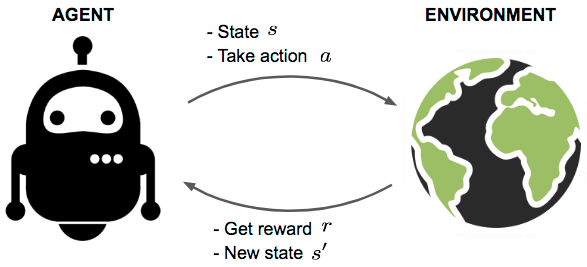
\includegraphics[width=2in]{include/rl_basic.png}
\end{center}

We first construct an ``exploratory'' policy that will be used to ``experience'' many samples from the space of possible transitions. As with any monte-carlo, the less representative the data is of the population, the more biased the inference will be. If our exploratory policy causes us to keep visiting the same subset of states, our optimization won't be based on data that reflects the complete nature of the MDP, so we may perform poorly if ever in a state outside where we explored, or miss out on discovering much better options. On the other hand, some states may not be important to the application because they are extremely unlikely to occur or are obviously highly suboptimal to pass through, in which case it makes sense to skip exploring them, especially if using function approximators with limited capacity. We don't want to waste time, memory, or reward becoming prepared for unimportant scenarios. This trade-off is called ``exploration vs exploitation.''\\

One simple exploratory policy that strikes a balance between exploration and exploitation is known as the ``$\epsilon$-greedy'' policy. It is a mixture distribution that selects a uniformly random action with small probability $\epsilon$ and the estimated optimal action with probability $1-\epsilon$.
\begin{gather*}
c\ \dist\ \mathcal{U}\big{(}[0, 1]\big{)}\\
\pi_\epsilon(a_t|s_t, c) \coloneqq \begin{cases} \mathcal{U}\big{(}\mathbb{A}\big{)} &\text{if}\ c < \epsilon \\ \hat{\pi}^*(a_t|s_t) &\text{else}\end{cases}
\end{gather*}

Using the $\epsilon$-greedy policy, most of the time we are ``greedy'' and exploit our current estimate of the optimal policy in hopes of moving towards more rewarding regions of the state space, but some small percent of the time we do something random to explore more. Even though $\epsilon$-greedy isn't always an effective exploratory policy, it highlights the core trade-off in a clear way: exploring means trying something that we probably haven't tried before (which might be harmful), while exploiting means following our estimate of the optimal policy $\hat{\pi}^*$ (which might be biased).\\

The dynamic programming principle expresses $\hat{\pi}^*$ as a maximization of an expectation of $\hat{V}^*$. However, computing expectations requires knowing the model probabilities. To get around this, instead of retaining an estimate of the value function, we'll retain an estimate of the expectation itself that we can improve by monte-carlo. Define the ``action-value function,''
\begin{equation*}
Q^*(s_t, a_t) \coloneqq E\big{(}r_{t+1} + \gamma V^*(s_{t+1}) | s_t, a_t\big{)}
\end{equation*}

Rewriting the dynamic programming principle and Bellman equation in terms of $Q^*$ we have,
\begin{gather*}
\bar{\pi}^*(s_t) = \argmax_{a_t} Q^*(s_t, a_t)\\
V^*(s_t) = \max_{a_t} Q^*(s_t, a_t)\\
\implies\ \ \ Q^*(s_t, a_t) = E\big{(}r_{t+1} + \gamma \max_{a_{t+1}} Q^*(s_{t+1}, a_{t+1}) | s_t, a_t\big{)}
\end{gather*}

Now, by maximizing our current estimate of $Q^*$ we can select useful actions for engaging the environment without explicitly computing an expectation. Meanwhile, each transition that we sample can be used to monte-carlo a fixed-point-iteration that improves our $Q^*$ estimate. This bootstrap method is known as ``Q-learning,'' shown here with $\epsilon$-greedy exploration,
\begin{align*}
&\text{Guess}\ \ \hat{Q}^*_0\\
&\forall\ i \in \mathbb{N}\ :\\
&\text{\tab Sample initialization}\ \ s_0\ \dist\ p(s_0)\\
&\text{\tab $\forall\ t \in \mathbb{T}$ :}\\
&\text{\tab \tab Sample policy}\ \ a_t\ \dist\ \begin{cases} \mathcal{U}\big{(}\mathbb{A}\big{)} &\text{if}\ \epsilon > c\ \dist\ \mathcal{U}\big{(}[0,1]\big{)} \\ \delta\big{(}a_t\ ;\ \argmax_{a} \hat{Q}^*_i(s_t, a)\big{)} &\text{else}\end{cases}\\
&\text{\tab \tab Sample environment}\ \ \{s_{t+1}, r_{t+1}\}\ \dist\ p{(}s_{t+1}, r_{t+1} | s_t, a_t{)}\\
&\text{\tab \tab Recurse}\ \ \hat{Q}^*_{i+1}{(}s_t, a_t{)} = r_{t+1} + \gamma \max_{a} \hat{Q}^*_i{(}s_{t+1}, a{)}
\end{align*}

Now that there is a monte-carlo involved, we must be concerned with the estimate's variance. To assist convergence, the $\hat{Q}^*$ update is usually low-pass filtered with a gradually decreasing ``learning rate'' $\alpha_i \in (0,1]$. This is sometimes called ``temporal difference (TD) learning.''
\begin{equation*}
\hat{Q}^*_{i+1}{(}s_t, a_t{)} = \hat{Q}^*_i{(}s_t, a_t{)} + \alpha_i \big{(}r_{t+1} + \gamma \max_{a} \hat{Q}^*_i{(}s_{t+1}, a{)} - \hat{Q}^*_i{(}s_t, a_t{)}\big{)}
\end{equation*}

Furthermore, the sampled transitions are often recorded in a database called ``experience,'' randomly ordered, and then reused for the $\hat{Q}^*$ update. This ``experience replay'' technique, like the low-pass filter, helps the estimate ``remember'' what it learned from previous transitions. But experience replay also helps with the moving target issue by uncorrelating the MDP dynamic and $\hat{Q}^*$ updates.\\

Note that the maximization in the $\hat{Q}^*$ update allows it to still learn the optimal $Q^*$ regardless of what policy is actually used to interact with / explore the environment. Thus Q-learning is deemed an ``off-policy'' method. A slight variant called ``SARSA'' is an ``on-policy'' method where the update simply uses $\hat{Q}^*_i{(}s_{t+1}, a_{t+1}{)}$ instead of $\max_{a} \hat{Q}^*_i{(}s_{t+1}, a{)}$.\\

Q-learning can of course be combined with function approximation as needed, $\hat{Q}^*(s_t,a_t) \approx \eta(s_t,a_t;\theta)$. Pro-tip: when the action space is small, it is often simpler to use $\eta(s_t;\theta) \mapsto \mathbb{A} \times \mathbb{R}$ so that the maximization over $\mathbb{A}$ only requires one forward pass of $\eta$.\\

Notice that the action-value function is the expected total reward for starting at state $s_t$, using action $a_t$, and from then on acting according to the optimal policy. That is,
\begin{equation*}
Q^*(s_t, a_t) = E_{\pi^*}(G_t | s_t, a_t)
\end{equation*}

The Bellman equation can be understood as using the Markov property to ``roll'' the MDP objective $E_{\pi^*}(G_t | s_t)$ into a recursion over a single transition. The switch to $Q^*$ can be understood as ``unrolling'' just the first step, so $Q$ might be called a ``1-step value function'' and $V$ a ``0-step value function.'' If the MDP is unrolled out to $n$ steps, then we arrive back at the original optimization over trajectories rather than transitions, i.e. no use of the dynamic programming principle.\\

Some approaches tackle the MDP this way, forming a monte-carlo approximation of the gradient of the entire $E_{\pi^*}(G_t | s_t)$ ``roll-out'' and using it to improve a parameterized policy distribution. These ``direct policy gradient'' methods are way less sample efficient than dynamic programming, but do not require global maximizations over $\mathbb{A}$. Interestingly, the dynamic programming approach can be combined with policy gradient methods in what are called ``actor-critic'' (AC) methods. The idea is to reduce the variance in the policy gradient estimates by honing a predictor of expected optimal value to be used as a ``baseline.'' AC methods are the current state-of-the-art.\\

To finish, lets allude to a few more places MDP theory can take us. So far, we have assumed that the current state was always available to choose an action based on. But what if the MDP had a noisy ``sensor'' $p(z_t|s_t,a_t)$ and our policy was restricted to being a function of only the sensor measurement history $\{z_\tau \in \mathbb{O}\ \ \forall \tau \leq t\}$? This is called a ``partially observed MDP'' (POMDP) or ``hidden Markov model'' (HMM). It elicits the idea of ``state estimator'' design.\\

Furthermore, our MDP seems to model a universe where there is only one agent choosing actions. Many situations have multiple agents competing with each other. Entering the realm of ``game theory,'' we can study ``minimax''-type problems and game theoretic versions of dynamic programming theory that handle how an agent should choose its actions knowing that the environment contains an adversary agent with its own objective in mind.\\

Lastly, there is always the modeling question of how to formulate real-world problems into a solvable MDP. It is often not clear what the state of a certain process even is, making the construction of a dynamic difficult. Even the reward function is not always easy to define for a given high-level desire. When it comes to the engineering side of MDP theory, these are often the most important questions.\\

%%%%%%%%%%%%%%%%%%%%%%%%%%%%%%%%%%%%%%%%%%%%%%%%%

\end{document}
